\documentclass{article}
\usepackage{tikz}
\usepackage{fullpage}
\begin{document}

\section*{Wiring diagram}
\section{Licence}
BBC:Micro:bit image from the microbit Educational Foundation at microbit.org (https://github.com/microbit-foundation/microbit-svg.git)

\begin{tikzpicture}
\node (microbit) at (0,0)
{
\def\svgwidth{0.4\columnwidth}
\input{fig/microbit-svg/microbit-drawing.pdf_tex}
};

% pin 0, 1, 2
\draw[line width=1em, color=black!30] (-2.50,-2.3) -- (-2.50,-19);
\draw[line width=1em, color=black!30] (-1.30,-2.3) -- (-1.30,-19);
\draw[line width=1em, color=black!30] (+0.03,-2.3) -- (+0.03,-19);
% +3V
\draw[line width=1em, color=red!70] (+1.37,-2.3) -- (+1.37,-19);
% GND
\draw[line width=1em, color=black!70] (+2.55,-2.3) -- (+2.55,-19);

% Motors
\node[rotate=-89] (m1) at (-6.5,-4){ 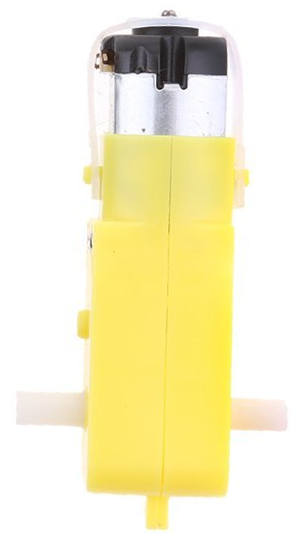
\includegraphics[scale=0.25]{fig/DCMotor-crop} };
\node[rotate=-89] (m2) at (-6.5,-7){ 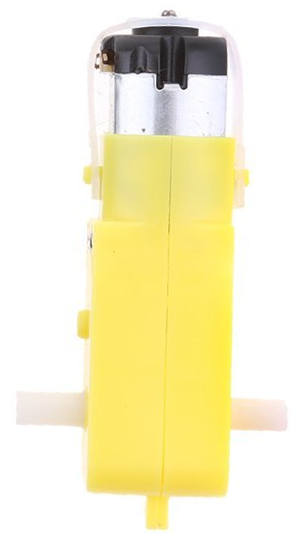
\includegraphics[scale=0.25]{fig/DCMotor-crop} };

% Empty slots left
\draw (-9,-9) rectangle (-4,-12);
\draw (-9,-12.5) rectangle (-4,-15.5);
\draw (-9,-16) rectangle (-4,-19);

% Empty slots right
\draw (4,-2) rectangle (9,-5);
\draw (4,-5.5) rectangle (9,-8.5);
\draw (4,-9) rectangle (9,-12);
\draw (4,-12.5) rectangle (9,-15.5);
\draw (4,-16) rectangle (9,-19);

\end{tikzpicture}

\end{document}
